\EnglishSourceFrame{GELFAND-P001385}{1}
\underline{5/X--87.}\qquad \underline{Gelfand seminar.}

\underline{A. Beilinson.}\quad \underline{Constructible sheaves} (continued).

\underline{Programme on sheaves.}

1. A sheaf; the category of sheaves.

2. Operations on sheaves: a) Gluing over an open cover

\hspace{2em}b) Gluing an open and a closed subset

\hspace{2em}c) Direct and inverse images.

3. Locally constant sheaves.

4. Combinatorial [crossed out: \EnglishUnclear{GELFAND-P001385}{cancelled-upper}{constructible?}] sheaves $=$ representations of ordered sets.

5. Constructible sheaves.

6. Cohomology with coefficients in sheaves.

7. Poincar\'e--Verdier duality.

For items 1--5, see the previous notebook.

Sheaves form an \underline{abelian category}.

Let $\mathcal F,G$ be sheaves, and let a morphism
$\mathcal F\overset{\varphi}{\longrightarrow}G$ be given.

All morphisms form a vector space (over $\mathbb C$).

\underline{Definition 1.}

$\operatorname{Ker}\varphi\subset\mathcal F$ [beneath the formula: subsheaf]
\begin{equation*}
(\ker\varphi)(V)=\{a\in\mathcal F(V),\ \varphi(a)=0\}
\end{equation*}
$\operatorname{Coker}\varphi$ is the sheaf associated to the presheaf $C$ of the form
\begin{equation*}
C(V)=\operatorname{Coker}(\varphi\colon\mathcal F(V)\longrightarrow G(V))
\end{equation*}

\underline{Constructing a sheaf from a presheaf.}

Let $C$ be a presheaf.

Let $V$ be an open set, $V=\bigcup V_\alpha$, and suppose that
$a_\alpha\in C(V_\alpha)$ are given, compatible with one another:
$a_\alpha|_{V_\alpha\cap V_\beta}=a_\beta|_{V_\alpha\cap V_\beta}$.
Such a family determines a section of the sheaf. There is an identification of sections,
\EnglishUnclear{GELFAND-P001385}{lower-gluing}{iskhod.? [unexpanded source abbreviation: «исход.»]}
from different families.

$C^+$ is [crossed out: \EnglishUnclear{GELFAND-P001385}{cancelled-bottom}{this? / pred...? [unresolved source beginning]}]
the sheaf associated to $C$.


\EnglishSourceFrame{GELFAND-P001386}{unlabelled}
There is a map
$C\longrightarrow C^+$,
universal in the following sense:

\begin{center}
\begin{tikzcd}
C \arrow[r] \arrow[dr, "{\forall f}"'] & C^+ \arrow[d, dashed, "{f^+\leftarrow\exists!}"] \\
& \mathcal F
\end{tikzcd}
\end{center}
[Beside $\mathcal F$ is written: sheaf.]

$\forall$ maps $f\colon C\longrightarrow\mathcal F$
[beneath $\mathcal F$: sheaf],
$\exists!\ f^+\colon C^+\longrightarrow\mathcal F$ such that the diagram commutes.

\underline{Exercise 1.}
[Crossed out: \EnglishUnclear{GELFAND-P001386}{cancelled-exercise}{pro...? [unresolved source beginning]}]
Construct $C^+$.

There are maps
\begin{equation*}
\operatorname{Ker}\varphi\overset{\alpha}{\longrightarrow}\mathcal F
\overset{\varphi}{\longrightarrow}G
\overset{\beta}{\longrightarrow}\operatorname{Coker}\varphi
\end{equation*}

\underline{Exercise 2.}\quad $\operatorname{Ker}\beta=\operatorname{Coker}\alpha$

An exact sequence of sheaves is defined naturally.

\underline{Exercise 3.}\quad The sequence $\mathcal F_1\longrightarrow\mathcal F_2\longrightarrow\mathcal F_3$
is exact $\Longleftrightarrow\forall x\in X$
the sequence $\mathcal F_{1x}\longrightarrow\mathcal F_{2x}\longrightarrow\mathcal F_{3x}$ is exact.

(Consider the inclusion $x\overset{i_x}{\longrightarrow}X$; then the stalk $\mathcal F_x$ at $x$
has the form $\mathcal F_x=i_x^*\mathcal F$.)

\underline{Definition 2 (Flasque sheaf)}

A sheaf $\mathcal F$ is called flasque if every section over an open set $V$ extends
to a section over all of $X$, i.e. $\forall$ open $V\subset X$,
\begin{equation*}
\mathcal F(X)\longrightarrow\mathcal F(V)
\end{equation*}
is an epimorphism.

\EnglishSourceFigure{GELFAND-P001386}{path-diagram}{Two oval regions, labelled $V_1$, $V_2$ above; the points marked inside them are joined by a wavy line without a clearly distinguishable arrow. Beneath are labels $s_1$, $s_2$ or $\xi_1$, $\xi_2$; the letter shapes require comparison with the original.}

% Supplement after the typed SourceFigure explanation. Requires graphicx/tikz.
\begin{center}
\begin{minipage}[t]{.46\linewidth}\vspace{0pt}\centering
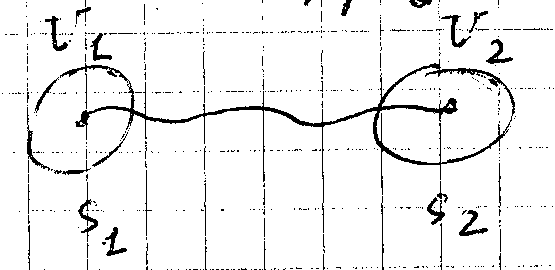
\includegraphics[width=\linewidth]{figures/gelfand-0151-p001386-path-original.png}\par\smallskip
{\footnotesize Original manuscript detail: \texttt{GELFAND-P001386}}
\end{minipage}\hfill
\begin{minipage}[t]{.50\linewidth}\vspace{0pt}\centering
{\footnotesize Partial typographic recreation}\par\smallskip
% Partial native recreation of GELFAND-P001386. No transport arrow is supplied.
% Preserve the visible break in the left oval; bottom labels remain candidates.
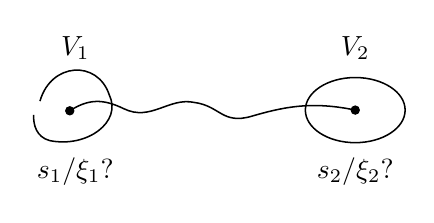
\begin{tikzpicture}[x=.88cm,y=.88cm,line width=.55pt]
\draw (-.43,.14) .. controls (-.27,.70) and (.40,.74) .. (.57,.23)
  .. controls (.76,-.16) and (.25,-.54) .. (-.29,-.43)
  .. controls (-.48,-.38) and (-.53,-.20) .. (-.52,-.06);
\draw (4.12,.01) ellipse (.72 and .47);
\draw (0,0) .. controls (.28,.18) and (.49,.17) .. (.78,.03)
  .. controls (1.17,-.16) and (1.43,.20) .. (1.80,.12)
  .. controls (2.17,.07) and (2.20,-.20) .. (2.62,-.08)
  .. controls (3.10,.06) and (3.50,.14) .. (4.12,.01);
\fill (0,0) circle (1.7pt);
\fill (4.12,.01) circle (1.7pt);
\node at (.08,.90) {$V_1$};
\node at (4.12,.90) {$V_2$};
\node at (.08,-.88) {$s_1/\xi_1$?};
\node at (4.12,-.88) {$s_2/\xi_2$?};
\end{tikzpicture}

\end{minipage}
\end{center}
\noindent{\small\textit{The left oval has a visible gap in its outline. The lower labels remain alternatives, and no direction is assigned to the wavy line. The drawing indicates the geometry only; it does not assert a transport map.}}


In locally constant sheaves one can transport sections [inserted above the line: (along a path)],
and therefore such sheaves are not \underline{flasque}.

\underline{Problem 4.}\quad $\Gamma$ is an [inserted above the line: finite] ordered set; introduce the topology
\begin{equation*}
\overline{x}:=\{y:\ y\leq x\}\quad\text{-- the closure of the point }x
\end{equation*}
a) Sheaves on $\Gamma$ $=$ representations of $\Gamma$.

b) Describe flasque sheaves on $\Gamma$.


\EnglishSourceFrame{GELFAND-P001387}{2}
c) The connection with combinatorial sheaves

Suppose that $X$ has a stratification; consider the map
\begin{tikzcd}[row sep=small]
X \arrow[d, "\pi"'] \\
\Gamma
\end{tikzcd}
(the point $x$ is sent to its stratum).

$\Gamma$ is the ordered set of strata.

[Caption beneath $\Gamma$:] Introduce the (Zariski) topology on $\Gamma$.

\underline{Assertion.}

\underline{$\forall$ combinatorial sheaves on $X$ are inverse images}
[crossed out: \EnglishUnclear{GELFAND-P001387}{cancelled-pullback}{sheaves? [source plural]}]
\underline{of sheaves on $\Gamma$}
(and conversely)
\begin{equation*}
\pi^*\colon\text{sheaves on }\Gamma\overset{\sim}{\longrightarrow}
\text{combinatorial sheaves on }X.
\end{equation*}

\underline{Exercise 5.}\quad a) Let
$0\longrightarrow\mathcal F_1\longrightarrow\mathcal F_2\longrightarrow\mathcal F_3\longrightarrow0$
be a short exact sequence of sheaves. Then the sequence of sections
\begin{equation*}
0\longrightarrow\mathcal F_1(X)\longrightarrow\mathcal F_2(X)\longrightarrow\mathcal F_3(X)
\end{equation*}
is exact.

b) If $\mathcal F_1$ is flasque, the sequence
\begin{equation*}
0\longrightarrow\mathcal F_1(X)\longrightarrow\mathcal F_2(X)\longrightarrow\mathcal F_3(X)\longrightarrow0
\end{equation*}
is exact.

\underline{A flasque resolution of a sheaf.}

\underline{Exercise 6}\quad Let $\mathcal F$ be a sheaf. Then 1) It can be embedded in
a flasque sheaf $\mathcal F\hookrightarrow G$.

2) Now construct the following exact sequence from $\mathcal F$:

\begin{center}
\begin{tikzcd}[column sep=small]
0 \arrow[r] & \mathcal F \arrow[r] & G^0 \arrow[rr] \arrow[dr] && G^1 \arrow[rr] \arrow[dr] && G^2 \arrow[r] & \ldots \\
&&& G^0/\mathcal F \arrow[ur, hook] && G^1/(G^0/\mathcal F) \arrow[ur, hook]
\end{tikzcd}
\end{center}
$G^i$ are flasque.

[Beneath the diagram:] and so on.

(a flasque resolution)

3) $\forall$ pairs of flasque resolutions can be embedded in a common third one.

\underline{Definition 3.}
\begin{equation*}
H^i(X,\mathcal F)=H^i(0\longrightarrow G^0(X)\longrightarrow G^1(X)\longrightarrow\ldots)
\end{equation*}
(Here $0\longrightarrow\mathcal F\longrightarrow G^0\longrightarrow G^1\longrightarrow\ldots$
is a flasque resolution of $\mathcal F$.)

On the right are the cohomology groups of a complex of vector spaces.

\underline{Definition 4.}\quad [Crossed out: Dual sheaf.]
\underline{Cohomology with compact support.}

Suppose that $X$ is locally compact. One can then consider
sections with compact support:
$\mathcal F_c(X)$ denotes sections with compact support on $X$.


\EnglishSourceFrame{GELFAND-P001388}{unlabelled}
\begin{equation*}
H_c^i(X,\mathcal F)=H^i(0\longrightarrow G_c^0(X)\longrightarrow G_c^1(X)\longrightarrow\ldots)
\end{equation*}

\underline{Definition 5.}\quad Dual sheaf.

Presheaf: $\mathcal F^*(V)=\mathcal F_c(V)^*$
(analogue of \EnglishUnclear{GELFAND-P001388}{dual-note}{distributions? [source genitive plural] / a distribution? [source singular ending]})

(the dual space in the sense of linear algebra)
\begin{equation*}
V_1\subset V_2\ \Rightarrow\ \mathcal F_c(V_1)\longrightarrow\mathcal F_c(V_2)
\quad\text{(inclusion)}
\end{equation*}
and $\mathcal F^*(V_2)\longrightarrow\mathcal F^*(V_1)$ arises.

\underline{Exercise 7.}

a) $\mathcal F^*$ is a sheaf if $\mathcal F$ is flasque.

b) If $\mathcal F^*$ is a sheaf, then $\mathcal F^*$ is flasque, i.e.
$\forall\underset{\text{open}}{V}\subset X$,
the map $\mathcal F^*(X)\longrightarrow\mathcal F^*(V)$ is surjective.


\EnglishSourceFrame{GELFAND-P001389}{unlabelled}
\underline{12.10.87.}\qquad \underline{Gelfand seminar.}

Vakhtangov told the actors in Princess Turandot to enter the stage in fashionable clothes
and change immediately (putting on a turban and so on). The stories of mathematics are eternal; only the language changes.

\underline{I. M. G.}\quad
\underline{On a combinatorial conjecture of Dyson concerning multinomial coefficients}

\underline{A paper from the thick green collection on combinatorics}

Consider
\begin{equation*}
F(x,a)=\prod_{i\neq j}\left(1-\frac{x_j}{x_i}\right)^{a_j},
\qquad a_j\in\mathbb N.\tag{1}
\end{equation*}
Find the constant term.

Dyson's conjecture (1962): the answer is
\begin{equation*}
\frac{(a_1+a_2\ldots+a_n)!}{a_1!a_2!\ldots a_n!}\tag{2}
\end{equation*}

In 1962, two (long) proofs were given in J. Math. Phys.

In 1970, a two-line proof in J. Math. Phys. by \EnglishUnclear{GELFAND-P001389}{author-name}{Wood? / Good? [source candidates: «Вуда» / «Гуда»]}.

\underline{Proof.}\quad Applying Lagrange's interpolation formula to the function
\EnglishUnclear{GELFAND-P001389}{interpolation-function}{$f\equiv0$}
and then setting $x=0$, we obtain
\begin{equation*}
\sum_j\prod_{i\neq j}\left(1-\frac{x_j}{x_i}\right)^{-1}=1\tag{3}
\end{equation*}

Multiplying by $F(x,a)$, we obtain


\EnglishSourceFrame{GELFAND-P001390}{unlabelled}
\begin{equation*}
\sum_j F(x,a_1,\ldots,a_{j-1},a_j-1,a_{j+1},\ldots,a_n)=F(x,a)\tag{4}
\end{equation*}

[Crossed out: \EnglishUnclear{GELFAND-P001390}{cancelled-let}{an illegible beginning.}]
Let $G(a)$ be the constant term. Then, from (4),
\begin{equation*}
G(a)=\sum G(a_1,\ldots,a_{j-1},a_j-1,a_{j+1},\ldots,a_n),\tag{5}
\end{equation*}
which gives a recurrence formula.

For $a_j=0$, we obtain
\begin{equation*}
G(a_1,\ldots,a_{j-1},0,a_{j+1},\ldots,a_n)
=G(a_1,\ldots,a_{j-1},a_{j+1},\ldots,a_n)\tag{6}
\end{equation*}
In addition,
\begin{equation*}
G(0)=1\tag{7}
\end{equation*}
Relations (5)--(7) are sufficient recurrence relations
to determine everything, and we obtain (2).

\underline{A. Veselov}

\underline{On geodesics on an ellipsoid and motion on a sphere}

Following Jacobi and others---1982: Kn\"orrer's observation, the equivalence of two problems.

[Two columns follow, separated by a brace-shaped line. Left column.]

1) $(Aq,q)=1$

Geodesics on an ellipsoid

Weierstrass found them in $\theta$-functions (1861).

The geodesic equation in the natural parameter:
\begin{equation*}
\ddot q=\lambda Aq\tag{1}
\end{equation*}
(acceleration $\sim$ the normal)

[Addition on the right, in parentheses:]
$\lambda$ is the Lagrange multiplier, found from the condition $(Aq,q)=1$.

[Right column.]

2) Another problem [crossed out: \EnglishUnclear{GELFAND-P001390}{cancelled-neumann}{C. Neu...?}]
C. Neumann (1859)

Motion with potential energy
\begin{equation*}
U(x)=\frac12(Ax,x)
\end{equation*}
on the sphere $|x|^2=1$.

Here the equation is
\begin{equation*}
x''=-Ax+ux\tag{$1'$}
\end{equation*}
or, in coordinates,
\begin{equation*}
x_i''=-a_i x_i+ux_i\tag{$1''$}
\end{equation*}
[On the right, a sign is crossed out: \EnglishUnclear{GELFAND-P001390}{equation-end}{$q$? / $u$?}]

[Continuation below the columns.]

Pass to another parameter:
\begin{equation*}
q''=-Aq+vq'\tag{2}
\end{equation*}
(the substitutions are written out explicitly, $\lambda\rightsquigarrow v$).

\EnglishUnclear{GELFAND-P001390}{constants-note}{Beneath $\lambda$ and $v$ are two short vertical strokes each, with const written beneath each pair.}

Then the substitution
\begin{equation*}
x=\frac{Aq}{|Aq|}\qquad\text{(Gauss substitution)}\tag{3}
\end{equation*}
takes solutions of problem 1) to solutions of problem 2)
(and \EnglishUnclear{GELFAND-P001390}{bijection-note}{vzaimoodn.? [unexpanded source abbreviation: «взаимоодн.»]}).

(H. Kn\"orrer, 1982)

Equation

[On the right:] Introduce an operator:
\begin{equation*}
L=-\frac{d^2}{dt^2}+u,\qquad Lx_i=a_i x_i\tag{4}
\end{equation*}
($x_i$ is an eigenfunction!!)


\EnglishSourceFrame{GELFAND-P001391}{12}
On the left:
\begin{equation*}
\widetilde L=-\frac{d^2}{dt^2}+v\frac{d}{dt}\tag{5}
\end{equation*}
(conjugate to $L$ by the Gauss substitution or the Miura substitution)

Kn\"orrer arrived at this through the Moser--Trubowitz isomorphism.

\underline{Consider problem 2).}

There are two symplectic forms.

\underline{Problem (I. M. G.)}\quad Given a symmetric matrix $A$ and a rank-one matrix $K$,
From the eigenvalues of $A+K$, how can one recover $K$? ($A$ is fixed.)

This is precisely Jacobi's formula.

\underline{V.}\quad For $n=2$, introduce new coordinates:
\begin{gather*}
M=[\dot x,x],\qquad\text{(angular momentum---cross product)}\\
p=x
\end{gather*}

$1^{\circ}$. The Lie--Berezin--Kirillov bracket
\begin{gather*}
\{M_i,M_j\}=\varepsilon_{ijk}M_k\\
\{M_i,p_j\}=\varepsilon_{ijk}p_k\\
\{p_i,p_j\}=0
\end{gather*}
The Hamiltonian
\begin{equation*}
2H=M^2+(Ap,p)
\end{equation*}
Then
\begin{equation*}
\begin{cases}
\dot M_i=\{M_i,H\}\\
\dot p_i=\{p_i,H\}
\end{cases}
\qquad\text{-- Neumann's equations}
\end{equation*}

\underline{Second bracket}
\begin{gather*}
\varepsilon_{ijk}a_kM_k=\{M_i,M_j\}\\
\varepsilon_{ijk}a_kp_k=\{M_i,p_j\}\\
\varepsilon_{ijk}M_k=\{p_i,p_j\}
\end{gather*}
The Hamiltonian $F=\frac12p^2$

\underline{I. M. G.}\quad This coincides with what Arnold described

(see the previous notebook).

The system is Hamiltonian with respect to both.


\EnglishSourceFrame{GELFAND-P001392}{unlabelled}
\underline{A. Beilinson.}\quad \underline{Constructible sheaves} (continued)

Representations of a partially ordered set $\Longleftrightarrow$
[crossed out: \EnglishUnclear{GELFAND-P001392}{cancelled-equivalence}{constructible?}]
combinatorial sheaves

\begin{center}
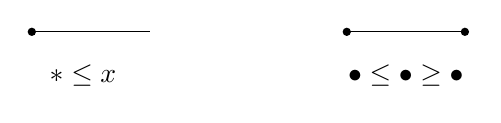
\begin{tikzpicture}
\draw (0,0) -- (1.5,0);
\fill (0,0) circle (1.5pt);
\node at (0.65,-0.55) {$\ast\leq x$};
\draw (4,0) -- (5.5,0);
\fill (4,0) circle (1.5pt);
\fill (5.5,0) circle (1.5pt);
\node at (4.75,-0.55) {$\bullet\leq\bullet\geq\bullet$};
\end{tikzpicture}
\end{center}

A combinatorial sheaf is a sheaf constant on each stratum.

\underline{Homological algebra.}

$\mathcal A$ is an abelian category (for example, sheaves over a given space or modules).

$C(\mathcal A)$ is the category of complexes over $\mathcal A$.

One needs to know the \underline{derived category} (Verdier, 1961).

Objects \EnglishUnclear{GELFAND-P001392}{objects-mark}{crossed-out ``from''? / a membership sign?}
$C(\mathcal A)$
\begin{gather*}
\ldots\longrightarrow X^i\overset{d}{\longrightarrow}X^{i+1}
\overset{d}{\longrightarrow}X^{i+2}\longrightarrow\ldots\\
d^2=0
\end{gather*}
Morphisms are morphisms of complexes (families of morphisms
\begin{tikzcd}[row sep=small]
X^i \arrow[d, "\varphi"'] \\
Y^i
\end{tikzcd} commuting with $d$).

$C(\mathcal A)$ is also an abelian category.

Bounded complexes (only finitely many terms $\neq0$): $C^b(\mathcal A)$

Bounded on the left or on the right: $C^{\pm}(\mathcal A)$
\begin{gather*}
C^+(\mathcal A)\text{ -- bounded on the left}\\
C^-(\mathcal A)\text{ -- bounded on the right}
\end{gather*}

The homotopy category $K(\mathcal A)$

The objects of $K(\mathcal A)$ are the same as those of $C(\mathcal A)$, and the morphisms are equivalence classes
of morphisms of $C(\mathcal A)$ under homotopy.
\begin{equation*}
\operatorname{Hom}_{K(\mathcal A)}(X^\bullet,Y^\bullet)
\end{equation*}

A morphism $X^\bullet\overset{\varphi}{\longrightarrow}Y^\bullet$ is [inserted above the line: such]
a family $\varphi^i\colon X^i\longrightarrow Y^i$ that the diagram commutes:

[On the left:]
\begin{center}
\begin{tikzcd}
X^{i-1} \arrow[r, "d"] \arrow[d, "{\varphi^{i-1}}"'] &
X^i \arrow[r, "d"] \arrow[d, "{\varphi^i}"] \arrow[dl, dashed, "{\psi^i}"'] &
X^{i+1} \arrow[d, "{\varphi^{i+1}}"] \arrow[dl, dashed, "{\psi^{i+1}}"'] \\
Y^{i-1} \arrow[r, "d"] & Y^i \arrow[r, "d"] & Y^{i+1}
\end{tikzcd}
\end{center}
[On the right:]
\begin{center}
\begin{tikzcd}
X^i \arrow[r, "d"] \arrow[d, "{\varphi^i}"'] & X^{i+1} \arrow[d, "{\varphi^{i+1}}"] \\
Y^i \arrow[r, "d"] & Y^{i+1}
\end{tikzcd}
\end{center}
[A wavy line goes around the left diagram above and on the right, then passes beneath the right diagram.]

$\varphi$ is called \underline{null-homotopic} if $\exists$ a family of maps
$X^i\overset{\psi^i}{\longrightarrow}Y^{i-1}$
such that
\begin{equation*}
\varphi^i=d\psi^i+\psi^{i+1}d\tag{1}
\end{equation*}


\EnglishSourceFrame{GELFAND-P001393}{13}
\underline{Exercise 1.}\quad Check that, for any family of maps $\psi^i$, the family (1)
defines a morphism of complexes, i.e. $d\varphi_i=\varphi_{i+1}d$.

\underline{Exercise 2.}\quad Morphisms homotopic to $0$ form an ideal, i.e. if
$\varphi$ is homotopic to $0$ and $\varphi_1$ is any morphism, then
$\varphi\circ\varphi_1$ is homotopic to $0$.

(The same is true for the composition $\varphi_2\circ\varphi$ with any morphism $\varphi_2$.)
\begin{equation*}
\operatorname{Hom}_{K(\mathcal A)}(X^\bullet,Y^\bullet)
=\operatorname{Hom}_{C(\mathcal A)}(X^\bullet,Y^\bullet)
/\bigl(\text{morphisms homotopic to }0\bigr)
\end{equation*}
There are obvious functors
\begin{equation*}
\mathcal A\longrightarrow C(\mathcal A)\longrightarrow K(\mathcal A)
\end{equation*}
The cohomology functor
\begin{equation*}
H^i\colon C(\mathcal A)\longrightarrow\mathcal A\qquad
\left(H^i(X^\bullet)=
\frac{\ker(d\colon X^i\longrightarrow X^{i+1})}
{\operatorname{Im}(d\colon X^{i-1}\longrightarrow X^i)}\right)
\end{equation*}

\underline{Exercise 3.}\quad Prove that $\exists!$ a functor
$H^i\colon K(\mathcal A)\longrightarrow\mathcal A$ such that
\begin{center}
\begin{tikzcd}
C(\mathcal A) \arrow[r] \arrow[dr, "{H^i}"'] & K(\mathcal A) \arrow[d, "{H^i}"] \\
& \mathcal A
\end{tikzcd}
\end{center}
The action of $H^i$ on morphisms is also defined in the obvious way.

\underline{Definition.}\quad $\varphi\colon X^\bullet\longrightarrow Y^\bullet$
[beneath the arrow: in the category $K(\mathcal A)$]
is called a \underline{quasi-isomorphism} if it induces an isomorphism
\begin{equation*}
H^i(X^\bullet)\longrightarrow H^i(Y^\bullet).
\end{equation*}

\underline{The derived category.}

\underline{Exercise 4.}\quad Suppose that there are three complexes
\begin{center}
\begin{tikzcd}
X^\bullet & & Y^\bullet \\
& Z^\bullet \arrow[ul, "\alpha"] \arrow[ur, "\beta"'] &
\end{tikzcd}
\end{center}
and morphisms, with $\alpha$ a quasi-isomorphism.

Then there exists a (commutative) diagram
\begin{center}
\begin{tikzcd}
& Z' & \\
X^\bullet \arrow[ur, "{\alpha'}"] & & Y^\bullet \arrow[ul, "{\beta'}"'] \\
& Z^\bullet \arrow[ul, "\alpha"] \arrow[ur, "\beta"'] &
\end{tikzcd}
\end{center}
[To the left of the lower part of the diagram, crossed out:
\EnglishUnclear{GELFAND-P001393}{cancelled-left}{in which? [abbreviated in the source]}.]

in which $\beta'$ is a quasi-isomorphism.

The same holds if one starts from the diagram
\begin{center}
\begin{tikzcd}
& Z' & \\
X^\bullet \arrow[ur, "{\alpha'}"] & & Y^\bullet \arrow[ul, "{\beta'}"']
\end{tikzcd}
\end{center}
with the quasi-isomorphism $\alpha'$.


\EnglishSourceFrame{GELFAND-P001394}{unlabelled}
\underline{The derived category} $D(\mathcal A)$

Objects $=$ the objects of $K(\mathcal A)$ (i.e. complexes)

Morphisms [inserted above the line: $X^\bullet\longrightarrow Y^\bullet$] are equivalence classes of diagrams
\begin{center}
\begin{tikzcd}
X^\bullet & & Y^\bullet \\
& Z^\bullet \arrow[ul, "\alpha"] \arrow[ur, "\beta"'] &
\end{tikzcd}
\qquad $\beta\alpha^{-1}$
\end{center}
($\alpha$ is a quasi-isomorphism)

under the equivalence relation \underline{generated}
by the \EnglishUnclear{GELFAND-P001394}{elementary-abbrev}{elm.? / elem.? [unexpanded source abbreviations]} relation.

[Crossed out: \EnglishUnclear{GELFAND-P001394}{cancelled-there}{There is? / If?}.]

(There is a functor $K(\mathcal A)\longrightarrow D(\mathcal A)$.)

\begin{center}
\begin{tikzcd}
X^\bullet & & Y^\bullet \\
& Z^\bullet \arrow[ul, "\alpha"] \arrow[ur, "\beta"'] & \\
& T \arrow[u, "\gamma"] &
\end{tikzcd}
\end{center}

\EnglishUnclear{GELFAND-P001394}{fraction-relation}{$\beta\alpha^{-1}\sim\beta\gamma(\alpha\gamma)^{-1}$?},
where $\gamma$ is a quasi-isomorphism.

\begin{center}
\begin{tikzcd}
X^\bullet & & Y^\bullet \\
& Z^\bullet \arrow[ul, "\alpha"] \arrow[ur, "\beta"'] &
\end{tikzcd}
\quad $\sim$ \quad
\begin{tikzcd}
X^\bullet & & Y^\bullet \\
& T \arrow[ul, "{\alpha\gamma}"] \arrow[ur, "{\beta\gamma}"'] &
\end{tikzcd}
\end{center}

These morphisms can now be composed.

\begin{center}
\begin{tikzcd}
X^\bullet & & Y^\bullet & & W \\
& Z^\bullet \arrow[ul] \arrow[ur] & & T \arrow[ul] \arrow[ur] & \\
& & S \arrow[ul] \arrow[ur] & &
\end{tikzcd}
\end{center}
[To the right of the lower part of the diagram, a left-pointing arrow with the caption:]
$\longleftarrow$ complete it \underline{by the lemma}.

The composition is the outer side of the diagram.

